\documentclass{tufte-handout}
% \documentclass{article}

%\date{28 March 2010} % without \date command, current date is supplied

% \geometry{showframe} % display margins for debugging page layout

\usepackage{graphicx} % allow embedded images
  \setkeys{Gin}{width=\linewidth,totalheight=\textheight,keepaspectratio}
  \graphicspath{{graphics/}} % set of paths to search for images
\usepackage{amsmath}  % extended mathematics
\usepackage{booktabs} % book-quality tables
\usepackage{units}    % non-stacked fractions and better unit spacing
\usepackage{multicol} % multiple column layout facilities
\usepackage{lipsum}   % filler text
\usepackage{fancyvrb} % extended verbatim environments
  \fvset{fontsize=\normalsize}% default font size for fancy-verbatim environments
\usepackage{listings}

% Standardize command font styles and environments
\newcommand{\doccmd}[1]{\texttt{\textbackslash#1}}% command name - - adds backslash automatically
\newcommand{\docopt}[1]{\ensuremath{\langle}\textrm{\textit{#1}}\ensuremath{\rangle}}% optional command argument
\newcommand{\docarg}[1]{\textrm{\textit{#1}}}% (required) command argument
\newcommand{\docenv}[1]{\textsf{#1}}% environment name
\newcommand{\docpkg}[1]{\texttt{#1}}% package name
\newcommand{\doccls}[1]{\texttt{#1}}% document class name
\newcommand{\docclsopt}[1]{\texttt{#1}}% document class option name
\newenvironment{docspec}{\begin{quote}\noindent}{\end{quote}}% command specification environment

\begin{document}

\title{MAE-253: Homework 2}
\author[John Karasinski]{John Karasinski}
\maketitle% this prints the handout title, author, and date

\section{Problem 1: The Cayley tree}
A Cayley tree is a symmetric regular tree emanating from a central node of degree $k$. Every node in the network has degree $k$, until we reach the nodes at the maximum depth $d$ that have degree one and are called the leaves of the network. For a Cayley tree of degree $k$ and depth $d$ calculate:

\subsection{a) How many vertices are exactly distance one from the center?}
3

\subsection{b) How many vertices are exactly distance two from the center?}
6

\subsection{c) How many vertices are exactly distance $l$ from the center?}
By induction, $k (k-1)^{l-1}$ for $l > 0$. For $l = 1, 2, 3, 4, 5$, for example, this leads to $3, 6, 12, 24, 48$.

\subsection{d) What is $n(l)$ the total number of vertices contained within distance $l$ from the central vertex? (Include the central vertex in this count).}

$n(l)$ is calculated by simply summing to distance $l$ and adding $1$,
\begin{align*}
n(l) = 1 + \sum_{l=1}^l k (k-1)^{l-1} = 1 + k \dfrac{1-(k-1)^l}{1-(k-1)}.
\end{align*}

\subsection{e) Present an argument that the Cayley tree has a small world diameter by showing that $d \sim \log{(n)}/\log{(k)}$. (It does not have to be rigorous, but show your reasoning.)}

Since the distance of any leaf node from the central node is $l$, the diameter of the Cayley tree is simply $d = 2l$. We then have
\begin{align*}
n(l) &= 1 + k \dfrac{1-(k-1)^l}{1-(k-1)} \\
     &= 1 + k \dfrac{1-(k-1)^{(d/2)}}{1-(k-1)} \\
\end{align*}
Plugging in $k=3$ and solving for $d$ leads to
\begin{align*}
n &= 1 + 3 (2 ^{d/2} - 1) \\
(\dfrac{n - 1}{3}) + 1 &= 2 ^{d/2} \\
\ln((\dfrac{n - 1}{3}) + 1) &= \dfrac{d}{2} ln(2) \\
\dfrac{2}{\ln{(2)}} \ln((\dfrac{n - 1}{3}) + 1) &= d
\end{align*}
For $n \gg 1$ we then have
\begin{align*}
d &= 2 \dfrac{\ln(n)}{\ln{(2)}}  \\
d & \approx 2 \dfrac{\ln(n)}{\ln{(k-1)}}
\end{align*}
which suggests a small world ($d \propto \ln{n}$).

\section{Problem 2: Finite size scaling}

Consider a network where node degree $k$ follows a power law degree distribution $p_k = (\gamma - 1)k^{-\gamma}$, with $\gamma > 1$. We will approximate $k$ as continuous and then let $P_K$ denote the cumulative distribution function (CDF) which is the probability a node will have degree less than or equal to $K$,
\begin{align*}
P_K = \int_1^K p_k dk.
\end{align*}

Here we will work out an estimate for the maximum node degree, $K_{max}$, that one would expect to see in a network of size $N$ with a power law degree distribution. Operationally, we define the expected value of $K_{max}$ for a network of size $N$ to be the value of degree when we expect only one node bigger than this value:
\begin{align*}
N (1 - P_{K_{max}} ) \approx 1.
\end{align*}

Using this show that $K_{max} \approx N^{1/(\gamma-1)}$ and evaluate the expression explicitly for $\gamma = 2,3,4$.

Integrating
\begin{align*}
P_K &= \int_1^K (\gamma - 1) k^{- \gamma} \\
    &= \dfrac{(\gamma - 1) k^{1 - \gamma}}{1 - \gamma} |_1^N \\
    &= 1 - K^{1-\gamma}
\end{align*}
Plugging this expression in to $N(1-P_{K_{max}}) \approx 1$, we have
\begin{align*}
N(1 - [1 - K_{max}^{(1-\gamma)}]) &\approx 1 \\
K_{max}^{(1-\gamma)} &\approx \dfrac{1}{N} \\
K_{max} &\approx \dfrac{1}{N}^{1/{(1-\gamma)}} \\
K_{max} & \approx N^{1/(\gamma-1)}
\end{align*}
Plugging in 2, 3, 4 into the formula for $K_{max}$ results in
\begin{align*}
K_{max}(2) & \approx N \\
K_{max}(3) & \approx N^{1/2} \\
K_{max}(4) & \approx N^{1/3}
\end{align*}
which indicates that larger values of $\gamma$ lead to lower values of $K_{max}$.

\section{Problem 3: Analysis of a real-world network}

For this problem you must find a data set of a real-world network. It could be a recommendation network of books constructed via amazon.com, a flight network for an air-line, a collaboration network of scientists or movie actors, a protein-interaction/gene-interaction network, a piece of the Amtrak rail network, a Facebook network, etc. The network should have somewhere between 200 to 1000 nodes.

\subsection{a) Describe your data set and where/how you obtained it. Is this a directed or undirected graph? Are there several components, or is it all one connected component?}

My dataset describes a network of all astronauts that have ever flown together in a spaceship that was either leaving or returning to Earth. Each node is an astronaut, and each edge relays that the two astronauts flew together. Since the astronauts flew together, this results in an undirected graph. I obtained the dataset from Wikipedia by crawling a list of all astronauts, and then did some minor manual cleansing of the data.

\subsection{b) How many nodes and edges are present? What is the average degree? (If it is a directed graph give values for both average in and out-degree.)}

There are 519 nodes and 2497 edges. The average degree is 9.6.

\subsection{c) Plot the degree distribution (again, if directed, plot both in and out-degree distributions). Identify the distribution that best fits your data, choosing from Gaussian, exponential, power law. (If you want to get more sophisticated, consider also power law with a cutoff and log normal distributions.)}

Three different functions were fit to the resulting degree distribution, and had the RMSE from the best fit and the true distribution was calculated. Though the Gaussian function performs slightly better than the exponential function, it requires an extra degree of freedom. As a result of this, the exponential function is considered to perform the best here.

\begin{table}[ht]
  \centering
  \fontfamily{ppl}\selectfont
  \begin{tabular}{lll}
    \toprule
    Name & Function & RMSE \\
    \midrule
    Gaussian    & $A e^{- { \frac{(x-B)^2 }{ 2 C^2} } }$ & 7.70 \\
    Power law   & $A x^B$ & 10.17 \\
    Exponential & $A B^x$ & 7.73 \\
    \bottomrule
  \end{tabular}
  \caption{Distributions fit to astronaut degree distribution with resulting RMSE.}
  \label{tab:normaltab}
  %\zsavepos{pos:normaltab}
\end{table}

\begin{figure}
  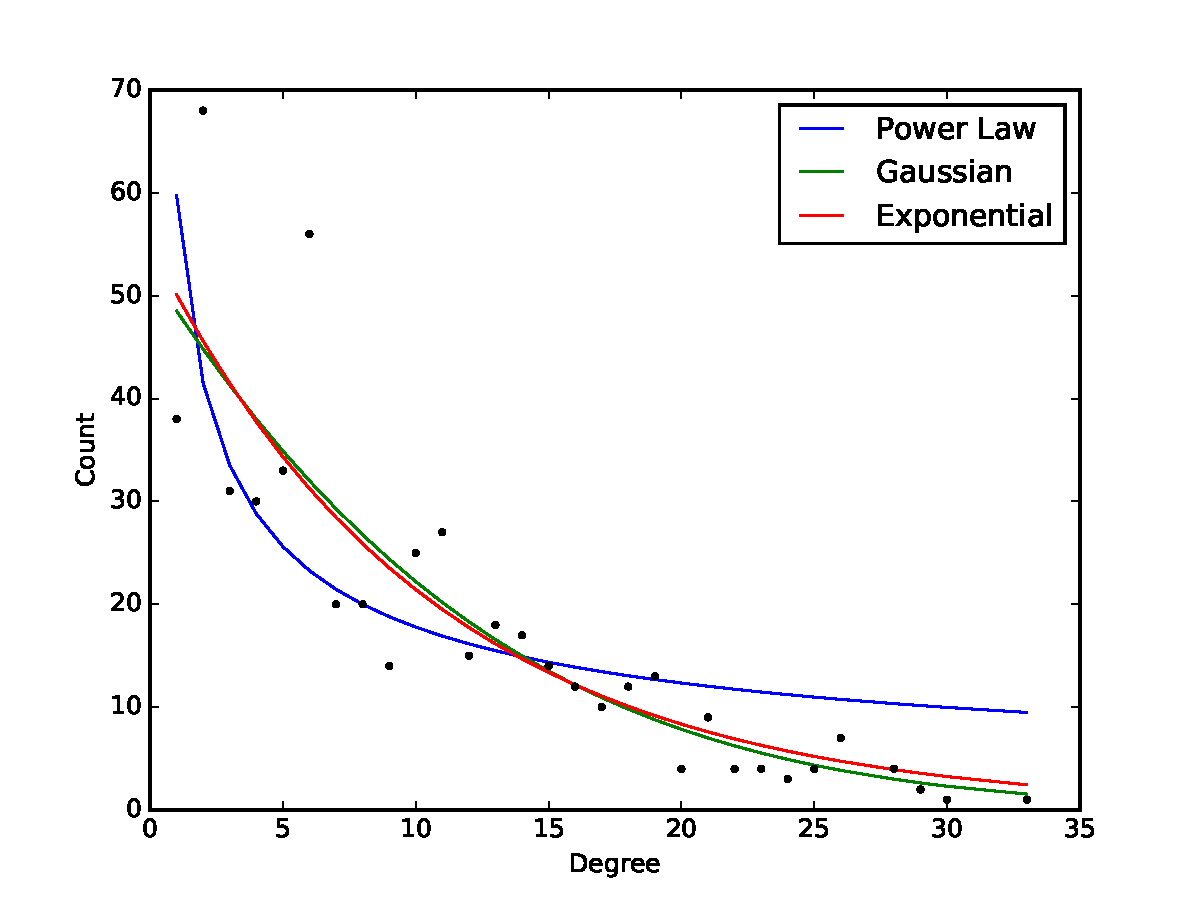
\includegraphics{fit_comparison.pdf}
%  \checkparity This is an \pageparity\ page.%
  \caption{Degree distribution with different distribution fits. The power law performs the worst, while the Gaussian and exponential fits perform nearly the same. In this case, the Gaussian performs lightly better.
  % \emph{Notice that this figure only takes up the main textblock width.}
  }
  \label{fig:textfig}
  %\zsavepos{pos:textfig}
  \setfloatalignment{b}
\end{figure}

\clearpage
\subsection{d) Visualize the network. Try to use color or size to display interesting attributes of your data (degree, age, high-clustering, etc). You may want to label the nodes with their identities.}

% \begin{figure*}[h]
%   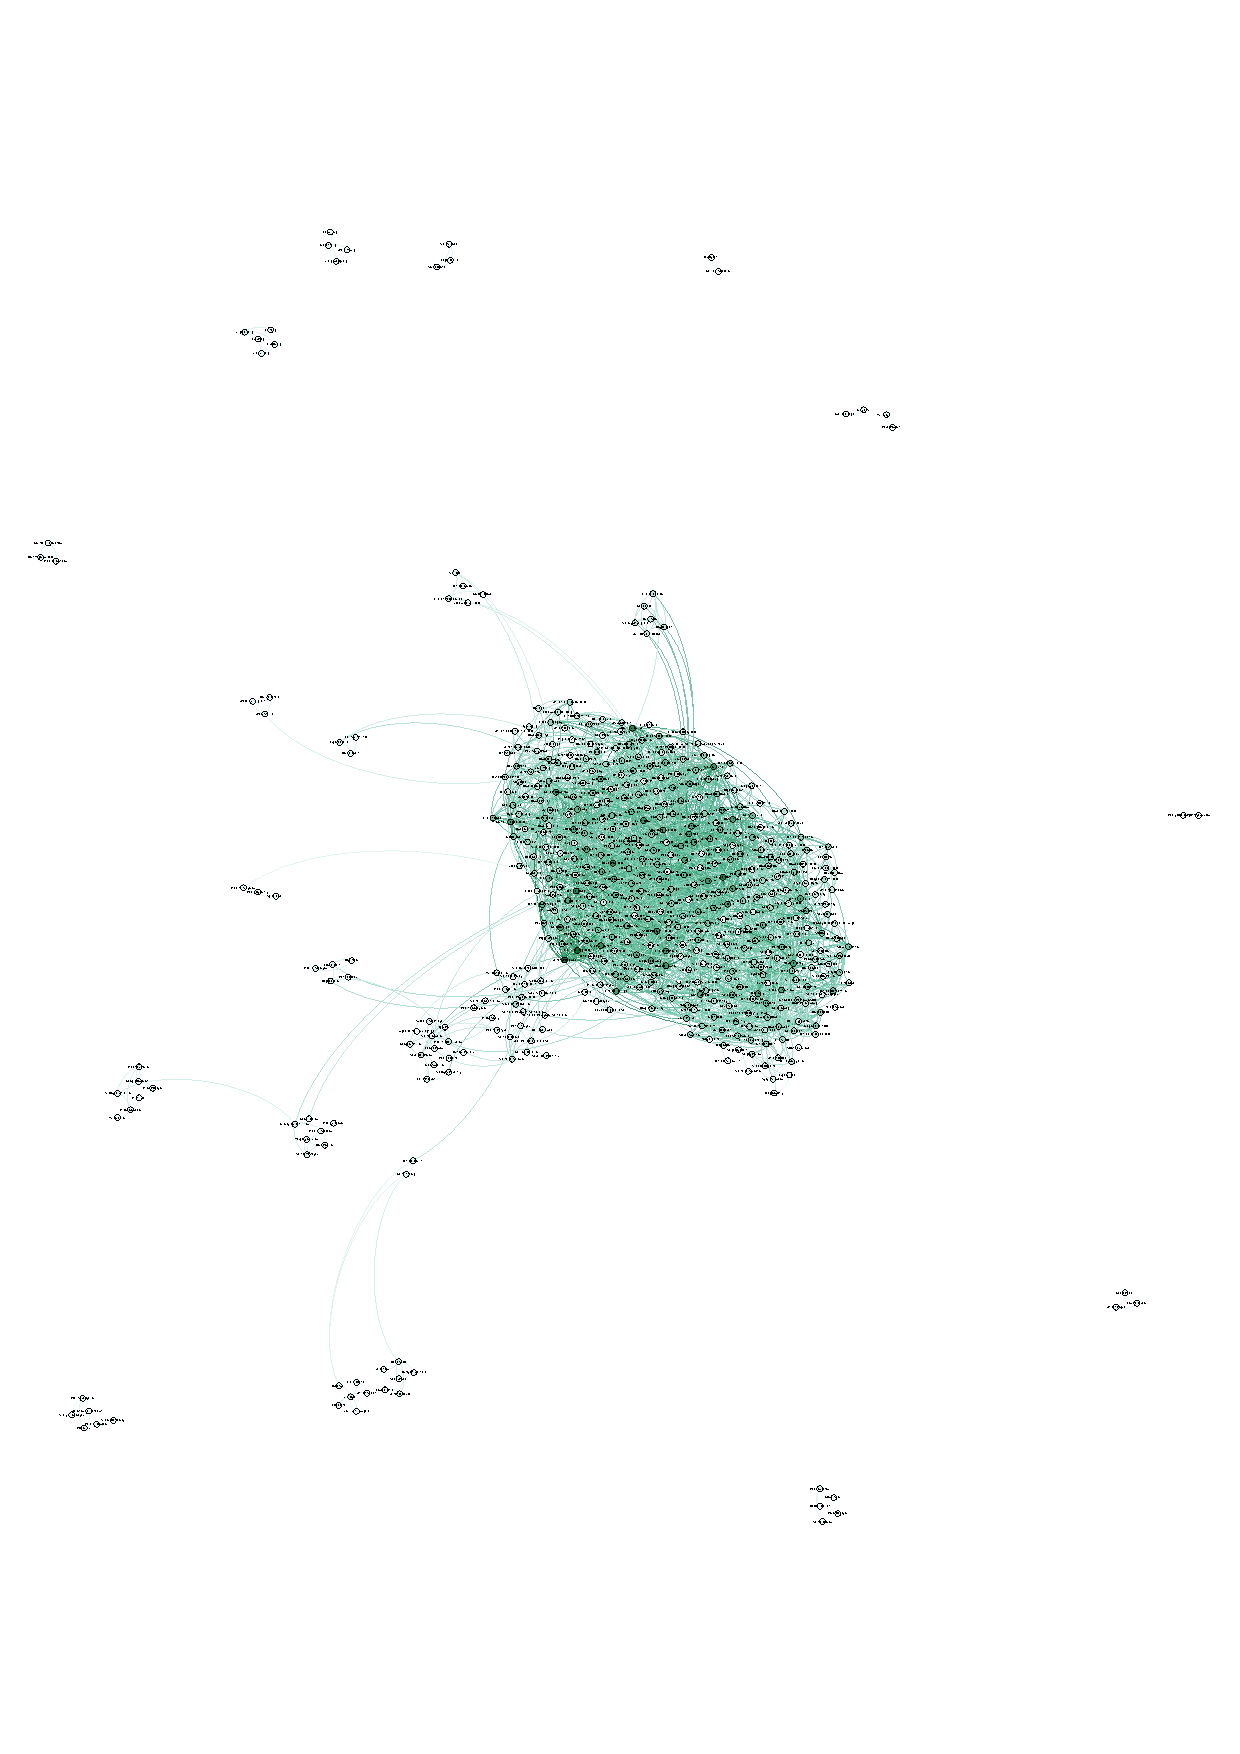
\includegraphics[height=0.5\textheight]{degree.pdf}%
%   \caption{This graph shows the degree of each node. Darker green shows a higher degree, and a lighter green in a lower degree.
%   % \emph{Notice that this figure takes up the full page width.}
%   }%
%   \label{fig:fullfig}%
% \end{figure*}

\begin{figure}
  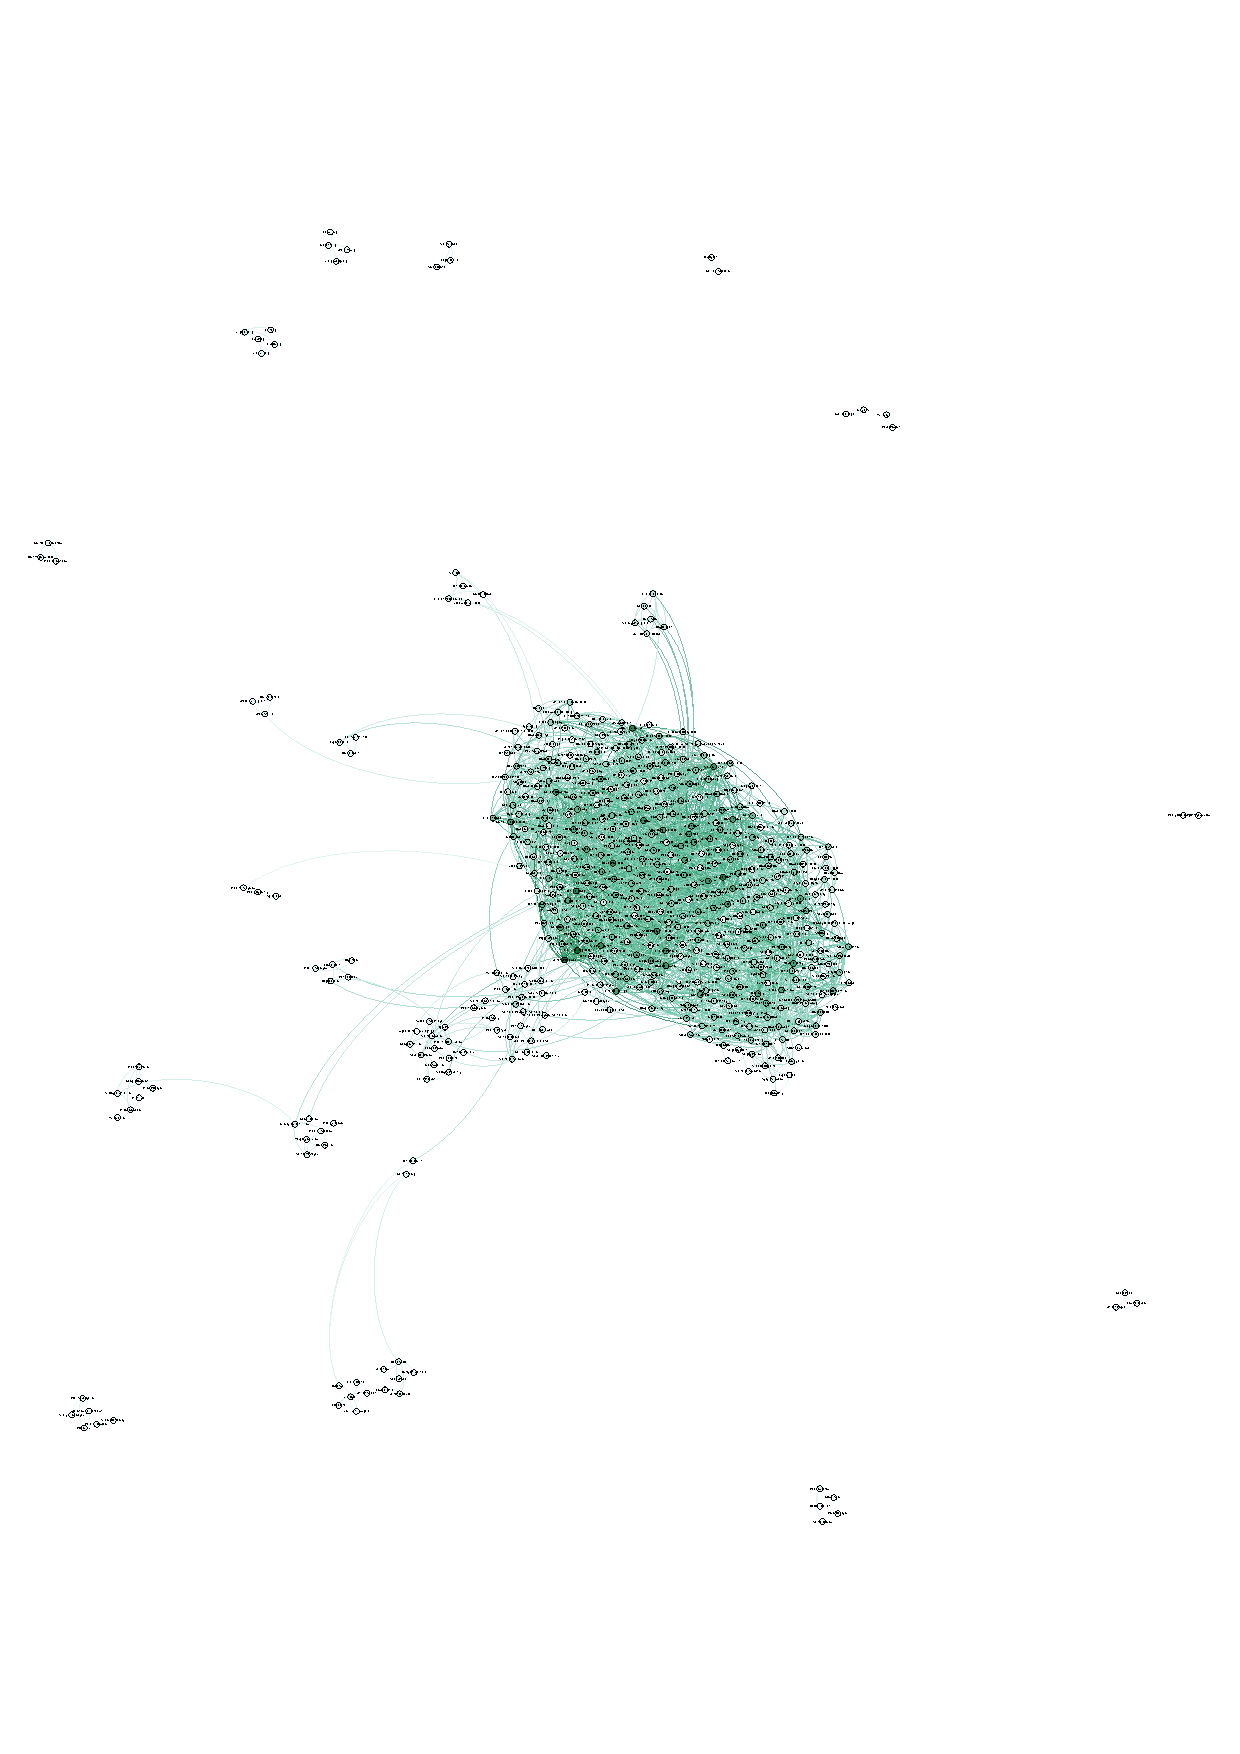
\includegraphics{degree.pdf}
%  \checkparity This is an \pageparity\ page.%
  \caption{This graph shows the degree of each node. Darker green shows a higher degree, and a lighter green in a lower degree. The nodes are labeled with the identities of the astronauts.
  % \emph{Notice that this figure only takes up the main textblock width.}
  }
  \label{fig:textfig}
  %\zsavepos{pos:textfig}
  \setfloatalignment{b}
\end{figure}


\clearpage
\subsection{e) Run a community detection algorithm on your network. How many communities did you find? What is the size distribution of the communities? Use the visualization of point d) and color code the communities. Can you interpret what you found?}

The community detection algorithm\footnote{Vincent D Blondel, Jean-Loup Guillaume, Renaud Lambiotte, Etienne Lefebvre, \emph{Fast unfolding of communities in large networks}, in Journal of Statistical Mechanics: Theory and Experiment 2008 (10), P1000} found 22 communities.

\begin{figure}
  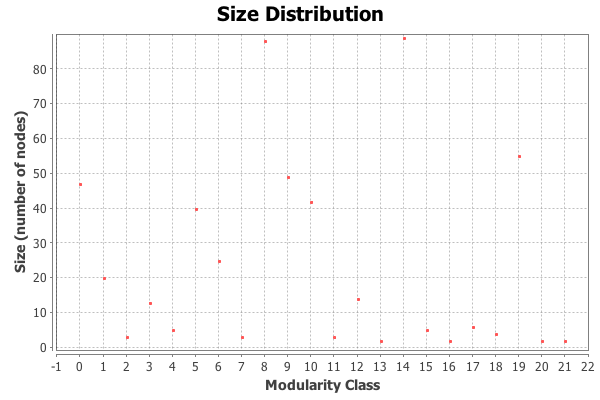
\includegraphics{communities-size-distribution.png}
%  \checkparity This is an \pageparity\ page.%
  \caption{Distribution of community sizes.
  }
  \label{fig:textfig}
  %\zsavepos{pos:textfig}
  \setfloatalignment{b}
\end{figure}

The small communities show groups of (mostly early) astronauts that only flew one mission. As such, they form a small community with the astronauts that they flew their single mission with. The blue community that comes off the primary cluster shows several of the Apollo missions, and the pink and orange communities just above it show groups of early Russian astronauts. The large central hub formed due to collaboration between US and Russian space agencies in the past few decades. Parts of the hub can be further decomposed into early/middle/late shuttle flights.

\begin{figure*}[h]
  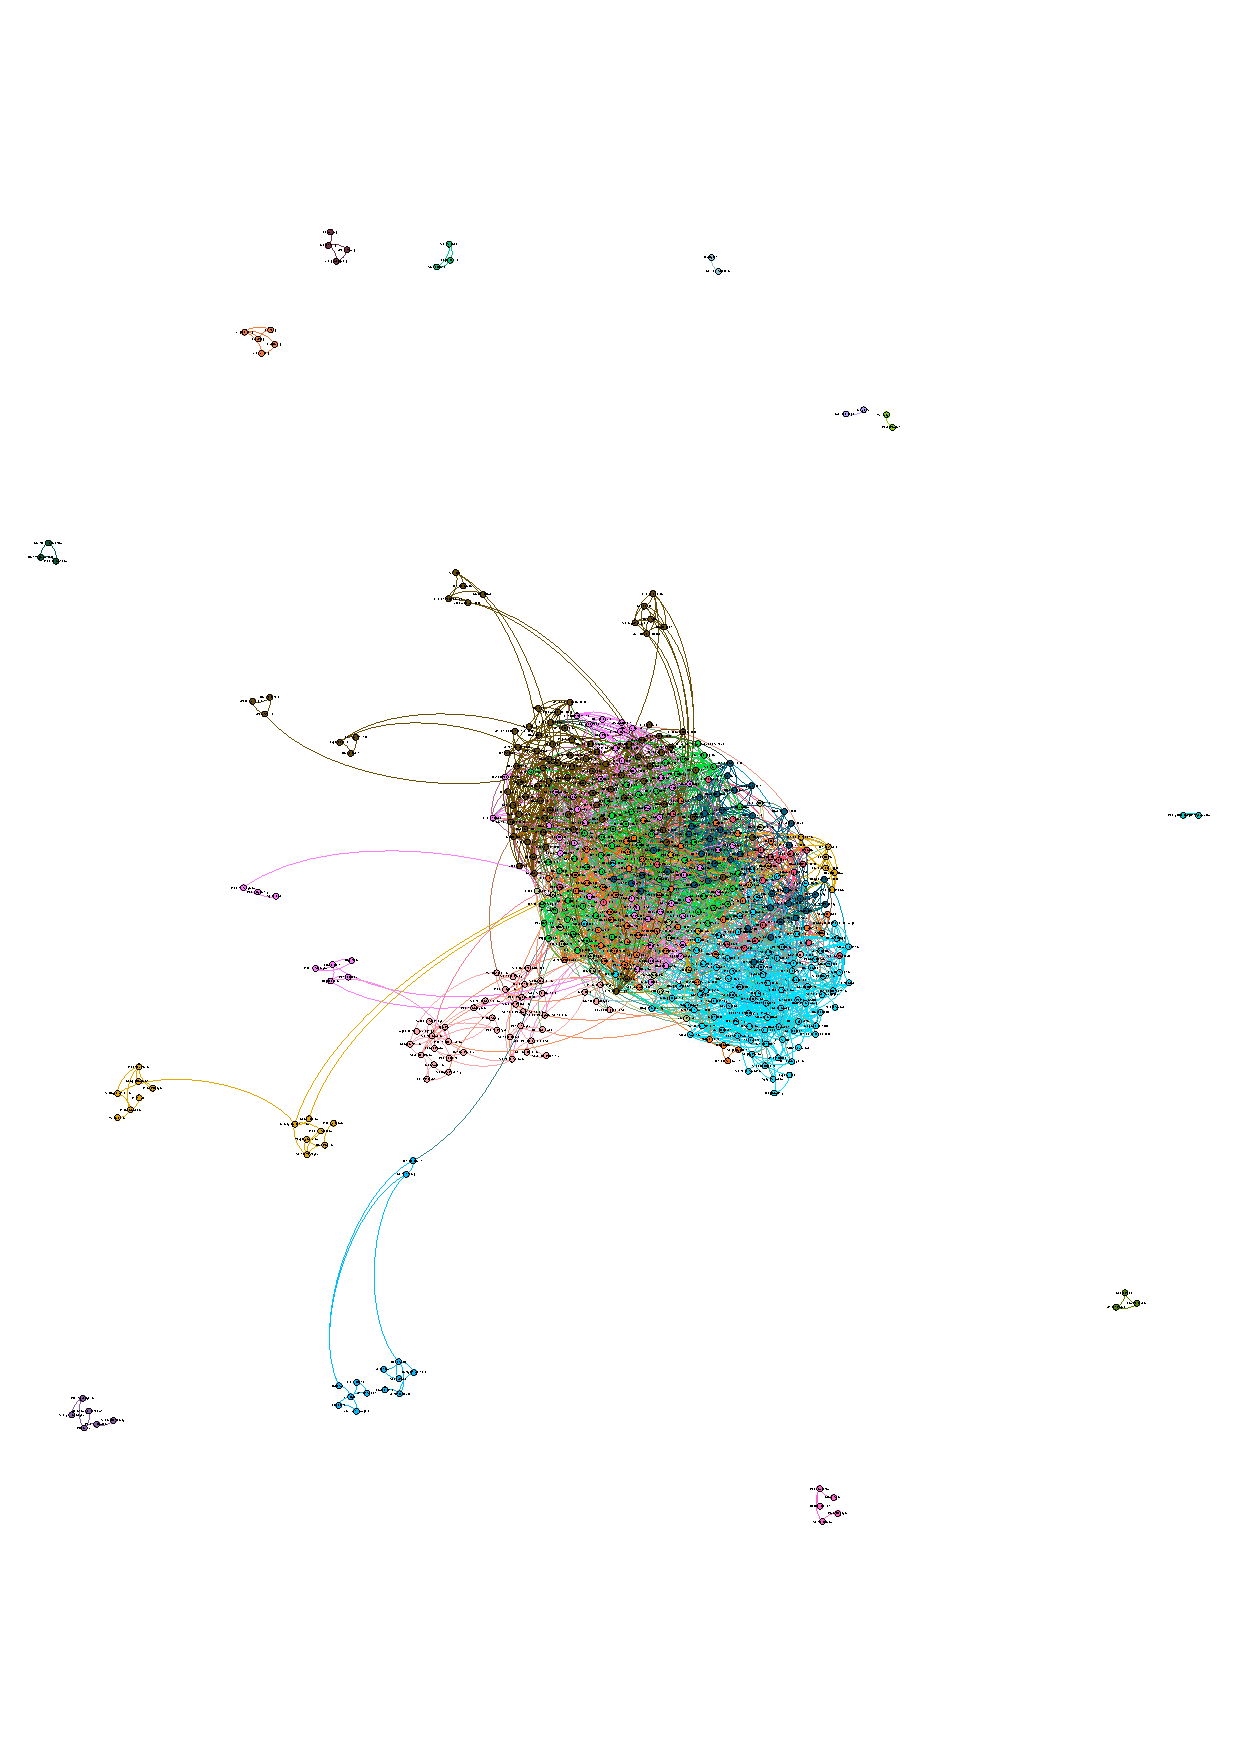
\includegraphics[width=\linewidth]{modularity.pdf}%
  \caption{This graph shows the community structure of the network. Each community is colored differently, and each node is labeled with the astronaut's name.
  % \emph{Notice that this figure takes up the full page width.}
  }%
  \label{fig:fullfig}%
\end{figure*}

% \begin{figure}
%   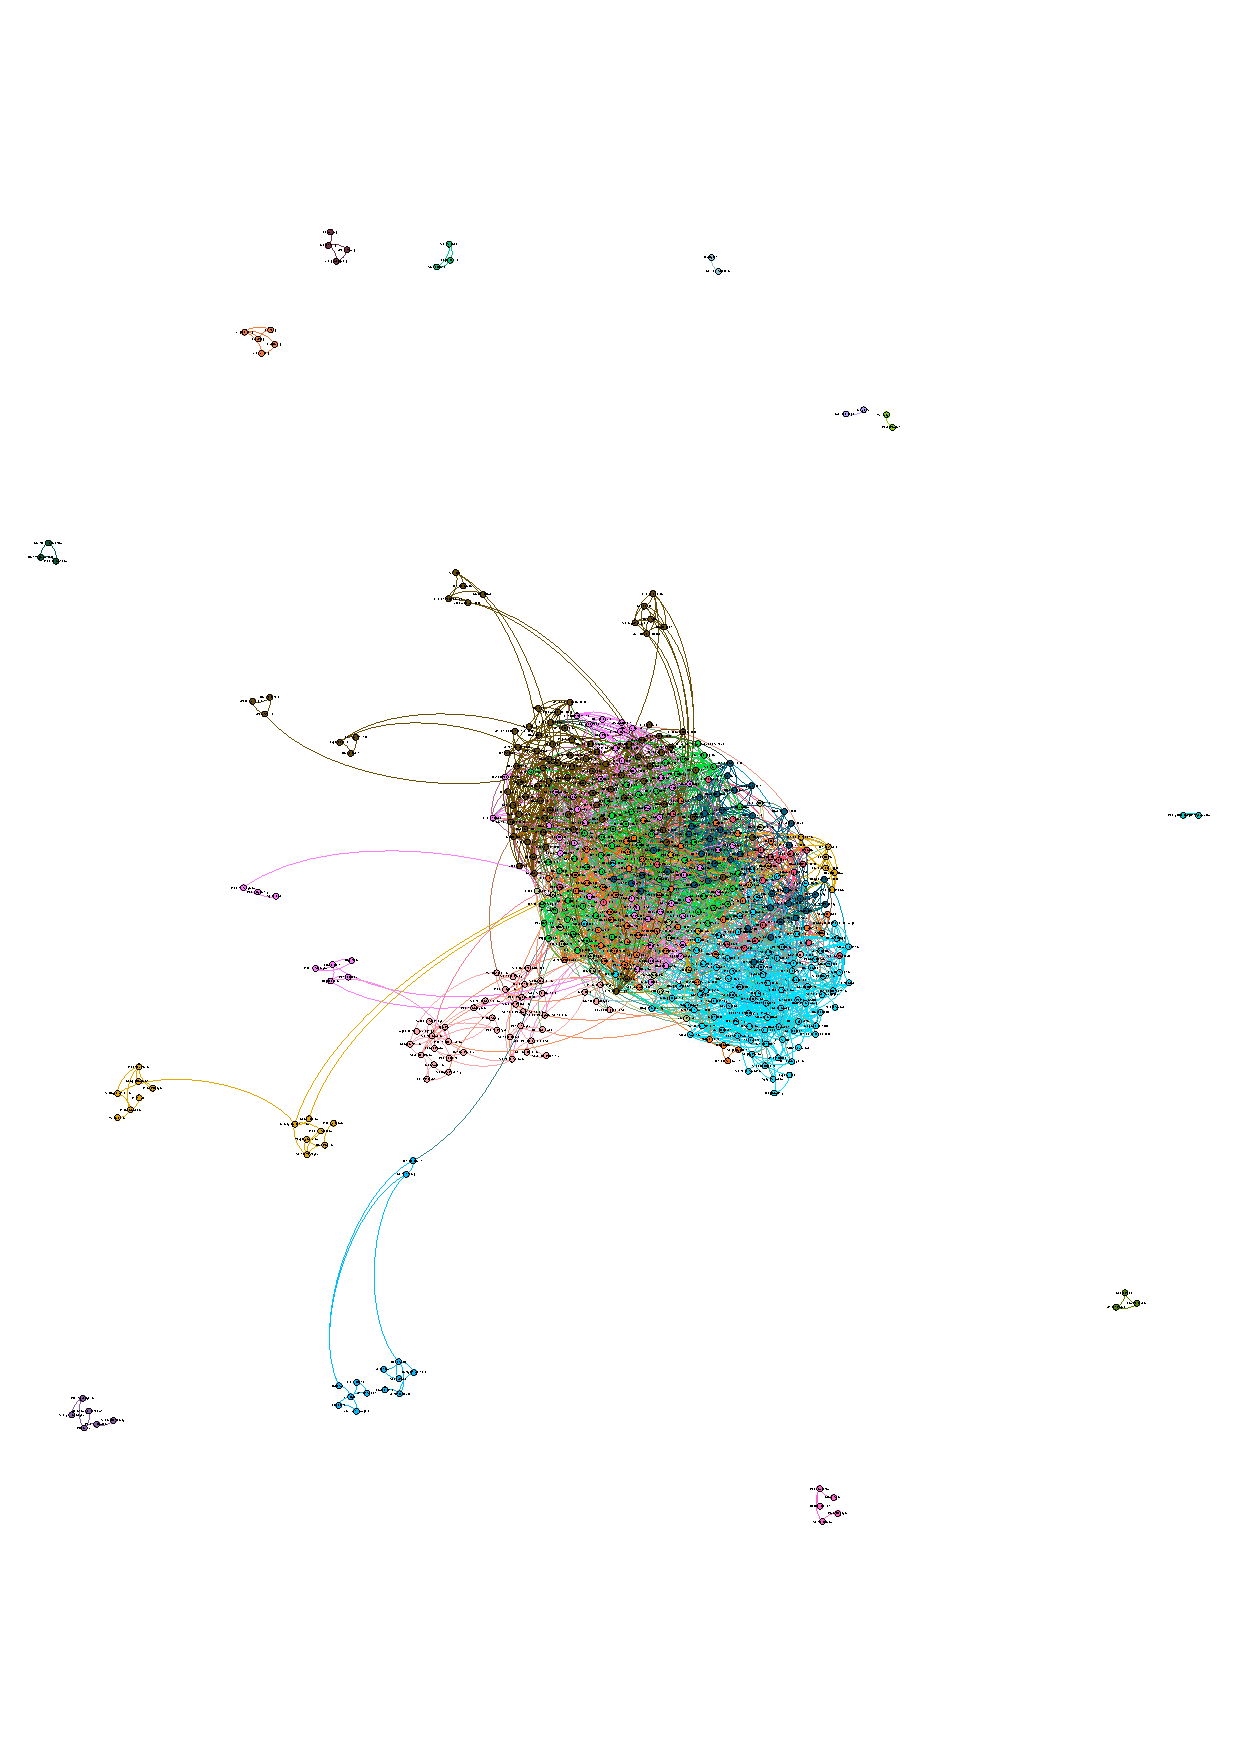
\includegraphics{modularity.pdf}
% %  \checkparity This is an \pageparity\ page.%
%   \caption{This graph shows the community structure of the network. Each community is colored differently.
%   % \emph{Notice that this figure only takes up the main textblock width.}
%   }
%   \label{fig:textfig}
%   %\zsavepos{pos:textfig}
%   \setfloatalignment{b}
% \end{figure}


\end{document}








